\documentclass[conference]{IEEEtran}
\IEEEoverridecommandlockouts
% The preceding line is only needed to identify funding in the first footnote. If that is unneeded, please comment it out.
\usepackage[noadjust]{cite}
\usepackage{filecontents}
\usepackage{amsmath,amssymb,amsfonts}
\usepackage{algorithmic}
\usepackage{graphicx}
\usepackage{textcomp}
\def\BibTeX{{\rm B\kern-.05em{\sc i\kern-.025em b}\kern-.08em
    T\kern-.1667em\lower.7ex\hbox{E}\kern-.125emX}}
\begin{document}

\title{Morphometry landmarks detection by convolutional neural network}

\author{\IEEEauthorblockN{Van Linh LE}
\IEEEauthorblockA{\textit{LaBRI - CNRS 5800, France} \\
\textit{ITDLU - Dalat University, Vietnam}\\
van-linh.le@labri.fr/ \\
linhlv@dlu.edu.vn}
\and
\IEEEauthorblockN{Marie BEURTON-AIMAR}
\IEEEauthorblockA{\textit{LaBRI - CNRS 5800} \\
\textit{Bordeaux University}\\
Talence, France \\
beurton@labri.fr}
\and
\IEEEauthorblockN{Akka ZEMMARI}
\IEEEauthorblockA{\textit{LaBRI - CNRS 5800} \\
\textit{Bordeaux University}\\
Talence, France \\
zemmari@labri.fr}
\and
\IEEEauthorblockN{Nicolas PARISEY}
\IEEEauthorblockA{\textit{IGEPP} \\
\textit{INRA 1349}\\
Le Rheu, France \\
nparisey@rennes.inra.fr}

}

\maketitle

\begin{abstract}
Morphometric analysis is general method applied on organisms and are useful to appraise the covariances between the ecological factors and the organisms(shape, size, form,...). In which, landmark-based morphometric is known as one of the approaches to analyze the characteristics of organisms. Finding enough the landmarks can give to the biologist a comprehensive description of organism shape. In this study, we propose a convolutional neural network (CNN) to predict the landmarks on biological images. The network is designed as a pipeline of the layers, it was trained with a set of manually landmarks examples. Then, the network is used to provide the morphometric landmarks on biological images automatically. The coordinates of predicted landmarks are evaluated by calculating the correlation coefficient with the manual coordinates which given by the biologists. Besides, the evaluations of the distances between predicted and manual landmarks are also given. The network is implemented by Python on Lasagne framework.
\end{abstract}

\begin{IEEEkeywords}
Morphometry, biological, landmarks, CNN
\end{IEEEkeywords}

\section{Introduction}
Morphometry analysis refers to measure the topography of an object, a notion that includes the shape and size. Morphometry analysis is generally applied to organisms. In biology, the biologist can work with several pieces of information from organisms such as lengths, widths, masses, angles,... to analyze the interaction of environment to the developmental of organisms. Besides the traditional information, the landmark is known as one of the characteristics to analyze the shape. Instead of collecting all information, the shape is determined by a finite set of points, called landmarks. The landmarks are the points that store the important information about the shape of the object, \textit{for example}, four corners of the rectangle are four landmarks of a rectangle. Normally, the landmarks are along on the outline of the object but in some special cases, it has been defined inside the object. Morphometry landmarks are a kind of points-of-interest, they are directly linked to the animal anatomy. In our study, the morphometric landmarks are specific points defined by the biologists. They are used in many biological studies and include the classification tasks. Manual landmarks identification is time-consuming and difficult to re-procedure. Therefore, a method that gives automatically the location of landmarks is very interesting.

This work introduces a method for automatic detection the landmarks on biological images. The main idea consists design and train a convolutional neural network\cite{lecun2010convolutional} with a set of manual landmarks. By this way, the trained network will be able to detect the morphometry landmarks on biological images. The dataset that used to study including 293 beetles images from Brittany lands. All the images are presented in RGB color with two dimensional. For each beetle, the biologists took images of five parts: \textit{left and right mandibles, head, body, and pronotum}. For every image, a set of landmarks has been manually determined by experts. In the last our work, a method has been presented to determine the landmarks on left and right mandibles\cite{le2017maelab}. This method is based on the image processing techniques\cite{canny1986computational}, combining with principal component analysis\cite{shlens2014tutorial} and SIFT descriptor\cite{lowe2004distinctive}. In the context of this work, we work on the dataset of pronotum images (Fig.\ref{figpronotum}). For each pronotum image, a set of 8 manual landmarks have been set by the biologists. The coordinates of manual landmarks were used as the input to train the network. During the first phase, a number of 260 images and their manual landmarks were used to train and validate the network. The remaining images were used to evaluate the output model of the network in the second phase.
\begin{figure}[htbp]
	\centerline{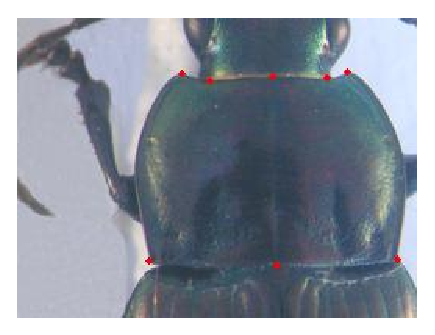
\includegraphics[scale=0.8]{images/pronotum}}
	\caption{An example of pronotum with manual landmarks}
	\label{figpronotum}
\end{figure}

In the next section, we study several related works to determine the landmarks on 2D images by CNN. Section 3 presents the architecture of the network, its parameters, and the implementation. All the experiments and analysing the results will be detailed in section 4.
\section{Related works}
In recent years, deep learning is known as a solution for computer vision literature. Using convolutional network to learn the vision features or to detect the important features on the images have achieved better results in many domains such as image classification\cite{krizhevsky2012imagenet}\cite{ciregan2012multi}, face detection and pose estimation\cite{li2015convolutional,lawrence1997face,farfade2015multi,osadchy2007synergistic}, handwritten detection\cite{lecun1990handwritten}\cite{graves2009offline} and key points (landmarks) identification \cite{sun2013deep,zhang2014facial,cintas2016automatic}. The landmarks are not only used in biology, they appear in many domains with many applications. Until now, most of the presented methods for identifying the landmarks that based on the image processing techniques\cite{palaniswamy2010automatic}\cite{kaur2015automatic}\cite{le2017maelab}. In this section, we introduce some studies that have applied the convolutional neural network to predict the landmarks automatically on 2D images.

In the field of facial keypoint detection, Yi Sun et al.\cite{sun2013deep} proposed cascaded convolutional networks to predict five facial points (points stay on the human face): \textit{left eye center, right eye center, nose, left mouth corner, and right mouth corner}. They cascade three levels of the convolutional networks to predict the facial points: In the first level, the networks are designed to predict several landmarks together by covering the whole face; the networks in the second and the third level are used to predict each landmark on the face. They take the patches centered at the predicted positions of previous levels as input and try to improve the accuracy of predicted positions. Zhanpeng Zhang et al\cite{zhang2014facial} proposed a \textit{Tasks-Constrained Deep Convolutional Network} to optimize facial landmarks detection. The model determined the facial landmarks with a set of related tasks such as head pose estimation, gender classification, age estimation, face recognition, or facial attribute inference. Firstly, all the images are used as the input, their output spaces the images into several tasks. Then, the network is applied to determine the landmarks on the images of each task. 

In biology field, Cintas et al\cite{cintas2016automatic} has introduced a network to predict the landmarks on human ears. The network was designed to receive the images with the size of $96 \times 96$ as the inputs. After training, the network has the ability to predict 45 landmarks and semi-landmarks on human ears. In their proposed architecture, the network with three times repeated of a structure includes two convolutional layers with the filters, followed by maximum pooling and dropout layers. The structures then adding two full-connected layers and a dropout layer. At the end, an output layer with 90 output units corresponding with 45 landmarks is hired to provide the position of the predicted landmarks.

\section{Method and implementation}
\label{sec3}
In previous section, we have introduced the methods using CNN to predict the landmarks. In this section, we describe the architecture of proposed network that use to predict the landmarks on biological images. Besides, the pratical techniques that using in deep learning are also recommended.
\subsection{Convolutional neural networks}
Deep learning allows computational model composed of multiple processing layers to learn representations of data with multiple levels of abstraction\cite{lecun2015deep}. Each layer extracts the representation of the input data from the previous layer and computes a new representation for the next layer. In the hierarchy of model, higher layers of representation enlarge aspects of the input that is important for discrimination and suppress irrelevant variations. Each level of representations is corresponding to the different level of abstraction. Almost the algorithms in deep learning learn are supervised (i.e classification) or unsupervised (i.e pattern analysis) practices. During training, it uses the forms of gradient descent to update the learnable parameters via backpropagation. The development of deep learning open the promises result of the artificial intelligent on hight dimensional data, therefore applicable to many domains: image recognition and classification\cite{krizhevsky2012imagenet,ciregan2012multi,szegedy2015going}, speech recognition\cite{mikolov2011strategies,hinton2012deep,sainath2013deep}, question answering\cite{bordes2014question} and language translation\cite{sutskever2014sequence}\cite{jean2014using}.

Convolutional neural networks (CNNs) contributes to resolve the state of the art in many computer vision such as classification\cite{krizhevsky2012imagenet}\cite{ciregan2012multi} or recognition\cite{li2015convolutional}\cite{tompson2014joint}. Normally, a CNN consists a number of connected layers. The layers of CNN has neurons arranged in three dimensions: \textit{width, height, and depth} with learnable parameters. The common layers in CNN are \textit{convolutional and pooling} layers. \textit{Convolutional} layer computes a dot product between their weights and a small region in the input. At the output, the results of connected local regions are combined. Convolution layer uses a set of learnable filters as parameters. Each filter is small spatially but extends the depth of the input. \textit{Pooling} layer uses to reduce the spatial size of the input. It usually to down-sampling the input. The main purpose of this layer is to reduce the computational cost in remaining layers, reducing the spatial of feature maps and control overfit.

From the beginning of deep learning until now, many deep learning frameworks have been developed. Almost the framework was served a specific aim and was open source. According to the written programming languages, the frameworks can be separated into two main groups: C++ and Python. In the group written by C++, the outstanding frameworks include Caffe\cite{jia2014caffe}, Deeplearning4j, Microsoft Cognitive Toolkit\cite{yu2014introduction}; whereas Keras\cite{chollet2015keras}, Theano\cite{2016arXiv160502688short} are known as the good frameworks that implemented by Python. Besides the main groups, we also have some frameworks that written in both programming languages such as Caffe2\cite{jia2014caffe}, TensorFlow\cite{abadi2016tensorflow}. In these frameworks, Caffe, Theano, and TensorFlow are known as good frameworks for convolutional neural networks. They provide the details of install, documentation with many examples in different domains such as classification, digit recognition.

Theano is an open source developed by machine learning group at the University of $Montr\acute{e}al$. It is a Python library that allows to define, optimize and evaluate mathematical expressions relating multi-dimensional arrays efficiently by using a Numpy package. Theano supports compiled on either CPU or GPU architectures. Lasagne\cite{lasagne} is a lightweight library in Theano. It allows to build and train the neural networks. In this work, we used Lasagne to implement the proposed neural network.
\subsection{Data and preprocessing data}
The images come from a collection of 293 beetles from Brittany lands. All the images are taken with the same camera under same conditions with a $3264 \times 2448$ resolutions. For each specific part, a set of manual landmarks has been determined by biologists, \textit{for examples, 8 landmarks for pronotum, 16 landmarks for the left mandible, 18 landmarks for right mandible}. In the content of this study, we work on pronotum part of beetle. The provided dataset contains 293 images, each image with 8 landmarks provided by biologists. The dataset was split into a training set with 260 images (training and validation) and a testing set of 33 images. During the training, the network learned the information through a pair of \textit{(image, landmarks)} in training set. At the testing phase, the image without landmarks was given to the trained network and the predicted landmarks will be given at the output.

Because the resolution of the image is large, it becomes a difficulty for the network. During training and testing, the images are down-sampling to the new resolution of $256 \times 192$. Certainly, the landmark coordinates of the image are also scaled to suit their new resolution. In practical when we work with CNN, convergence is usually faster if the average of each input variable over the training set is close to zero. Because the values of the pixels and the coordinates of the landmarks are positive. If we consider that we stay at a layer of the network, and the weights are updated by an amount proportional to $\delta x$($\delta$ is the scalar error at the layer and $x$ is the input vector). When the input vectors are positive, the updates of weights that feed into the layer will be the same sign($sign(\delta)$), it means that the weights can only all decrease or all increase together for a given input. That, if the weight vector change direction, it can only do by zigzagging which is inefficient and thus slow down learning. Therefore, it is good to shift the inputs so that the average over the training set is close to zero. Moreover, when the input is set closed with zero, it will more suitable with the sigmoid activation function\cite{lecun2012efficient}. Therefore, the brightness of the image is normalized to $[0,1]$, instead of $[0,255]$. And, the coordinates of the landmarks are normalized to $[-1,1]$, instead of $[0,256]$ and $[0,192]$ before giving to the network.
\subsection{Network architecture and training}
Three networks have been proposed and trained to perform the best architecture for automatically landmarking prediction. The networks consist several common layers in the neural network with different learnable parameters They receive the same input of $1 \times 256 \times 192$ to train but these have different number of layers. In this section, we introduce the architectures of the networks. And, we also present the process to improve the architecture from the beginning of designing.

Fig.\ref{figarch0} shows the architecture of the first network. In this model, it has been designed in a generic method: the layers in the network are very common as the other neural networks. The network consists three repeated-structure of a convolutional layer followed by a maximum pooling layer. The deep of convolutional layers increase from $32, 64,$ and $128$ with different size of the filter kernel: $3 \times 3$, $2 \times 2$, and $2 \times 2$. All the kernels of pooling layers have the same size of $2 \times 2$.  At the end, three full connected layers have been added to the network. The outputs of the full connected layers are $500, 500,$ and $16$, respectively. The output of the last full-connected layer corresponds to the number of the landmarks which we would like to predict. The training result shows that the architecture of this model is not enough good to solve the problem. It still simple and overfitting have appeared during training and validation. Then, number of outputs at full-connected layers have been modified from $500$ to $1000$ (the second model) to prevent the overfitting, but the result did not lead to better performances. 
%The CNN was designed and trained for performing an automatic landmarks detection on pronotum images. The network consists several common layers in the neural network with different learnable parameters. It takes a single channel pronotum image with the size of  $256 \times 192$ as the input. Before entering the network, the brightness of pixels in the image are normalized to $[0,1]$ and the coordinates of landmarks are normalized to $[-1,1]$.

\begin{figure}[htbp]
	\centerline{\includegraphics[scale=0.45]{images/architecture1}}
	\caption{The architecture of the first network}
	\label{figarch0}
\end{figure}

In the third network, we continued to improve the architecture of the last two models. Instead of changing the parameters, we have added four dropout layers to the network. These are considered as the good solution to prevent the overfitting. The idea of dropout is to randomly drop units from the neural network during training. It deters units from co-adapting too much. During training, dropout samples from an exponential number of different ``thinned" network. At test times, it is easy to approximate the effect of averaging the prediction of all thinned networks by simply using a single unthinned network that has smaller weights. This significantly reduces overfitting and gives major improvements over other regularization methods\cite{srivastava2014dropout}. Fig.\ref{figarch} shows the architecture of the third network. The first three dropout layers are supplemented to the repeated-structures followed the maximum pooling layers. It makes the structure become the consist of a convolution layer with square filter, followed with a \textit{maximum} pooling and dropout layer. The probability values used for dropout layers are $0.1$, $0.2$, and $0.3$. Actually, we keep the same value for the parameters of the convolutional, pooling and full-connected layers as the second one.

\begin{figure}[htbp]
	\centerline{\includegraphics[scale=0.45]{images/architecture3}}
	\caption{The architecture of the last network}
	\label{figarch}
\end{figure}

The remaining dropout layer is inserted between the first two full connected layers. The probability value of this layer is set to $0.5$. The output layer still contains 16 units corresponding to the coordinates of eight predicted landmarks. The detail of parameters at each layer are shown in Appendix section. 

Additional, the network is designed with a small sharing learning-rate and the momentum. They are updated over training time to fit with the remaining number of iterations. The implementation of this architecture used Python on Lasagne framework\cite{lasagne} which allows to train the network on GPU. The training process took around 3 hours using NVIDIA TITAN X cards. The design of the network is available on GitHub\footnote{It is freely obtained by request the authors.}.
\subsection{Overfitting problem}
The proposed network has a large number of learnable parameters. In addition, the size of the dataset is limited, this means that overfitting will occur during the training process. Because the network works on  gray-scale image and mostly the processes compute the value from the pixels. So, we have applied two rules to enlarge the size of the dataset.

The first rule was applied to change the value of each channel in the original image. According to this rule, a constant is adding to a channel of RGB image and for each time, we just change the value of one of three channels. For example, from an original RGB image, if we add a constant $c = 10$ to the red channel, we will obtain a new image with the values at red channel are greater than the red channel of original image a value of 10. By this way, we can generate three new RGB images from a RGB image.

The second rule is splitting the channels of RGB images. It means that we separate the channels of RGB into three gray-scale images. This work seems like right because the network works on single-channel images. At the end, we can generate six version from an image, the total number of images that used to train and validate is $260 \times 7 = 1820$ images (six versions and original image). The number of images that used for training and validation is split randomly by a ratio that has been set during setup the network.

%Besides enlarge the dataset, we also used dropout layers to prevent the overfitting. The idea of dropout is to randomly drop units from the neural network during training. It deters units from co-adapting too much. During training, dropout samples from an exponential number of different ``thinned" network. At test times, it is easy to approximate the effect of averaging the prediction of all thinned networks by simply using a single unthinned network that has smaller weights. This significantly reduces overfitting and gives major improvements over other regularization methods\cite{srivastava2014dropout}.
\section{Results}
The dataset has been built by the biologists. It includes the images and manual landmarks. So, we can use the manual landmarks coordinates as ground truth to evaluate the coordinates of predicted landmarks. In the context of deep learning, landmark prediction can see as the regression problem. Therefore, the quality metric is used to evaluate the results. In particular, we use root mean square error (RMSE) to compute the accuracy of the implemented architecture. To have the predicted coordinates of all landmarks in all the images, the network was trained many times with different training dataset and was tested on the corresponding test set.

Fig.\ref{figloss1} and \ref{figloss} show the training errors and the validation errors of a training time on the first and the third model. The blue curve presents RMSE on training set, the green curve presents the validation error. Clearly, the overfitting has appeared in the first model(Fig.\ref{figloss1}). Besides, the validation loss stabled from 2000 epochs while the training loss continued to decrease. This against with the losses of the third model. At the beginning, we see the variety between the losses but the training continue, the variety reduced and the overfitting problem have been solved.

\begin{figure}[htbp]
	\centerline{\includegraphics[scale=0.3]{images/loss_model_1}}
	\caption{Learning curves of the first model.}
	\label{figloss1}
\end{figure}
\begin{figure}[htbp]
	\centerline{\includegraphics[scale=0.35]{images/loss_v16}}
	\caption{Learning curves of the last model.}
	\label{figloss}
\end{figure}

Fig.\ref{figrsexample} shows the predicted landmarks on an unseen image in the test set by the thrid model. 

\begin{figure}[htbp]
	\centerline{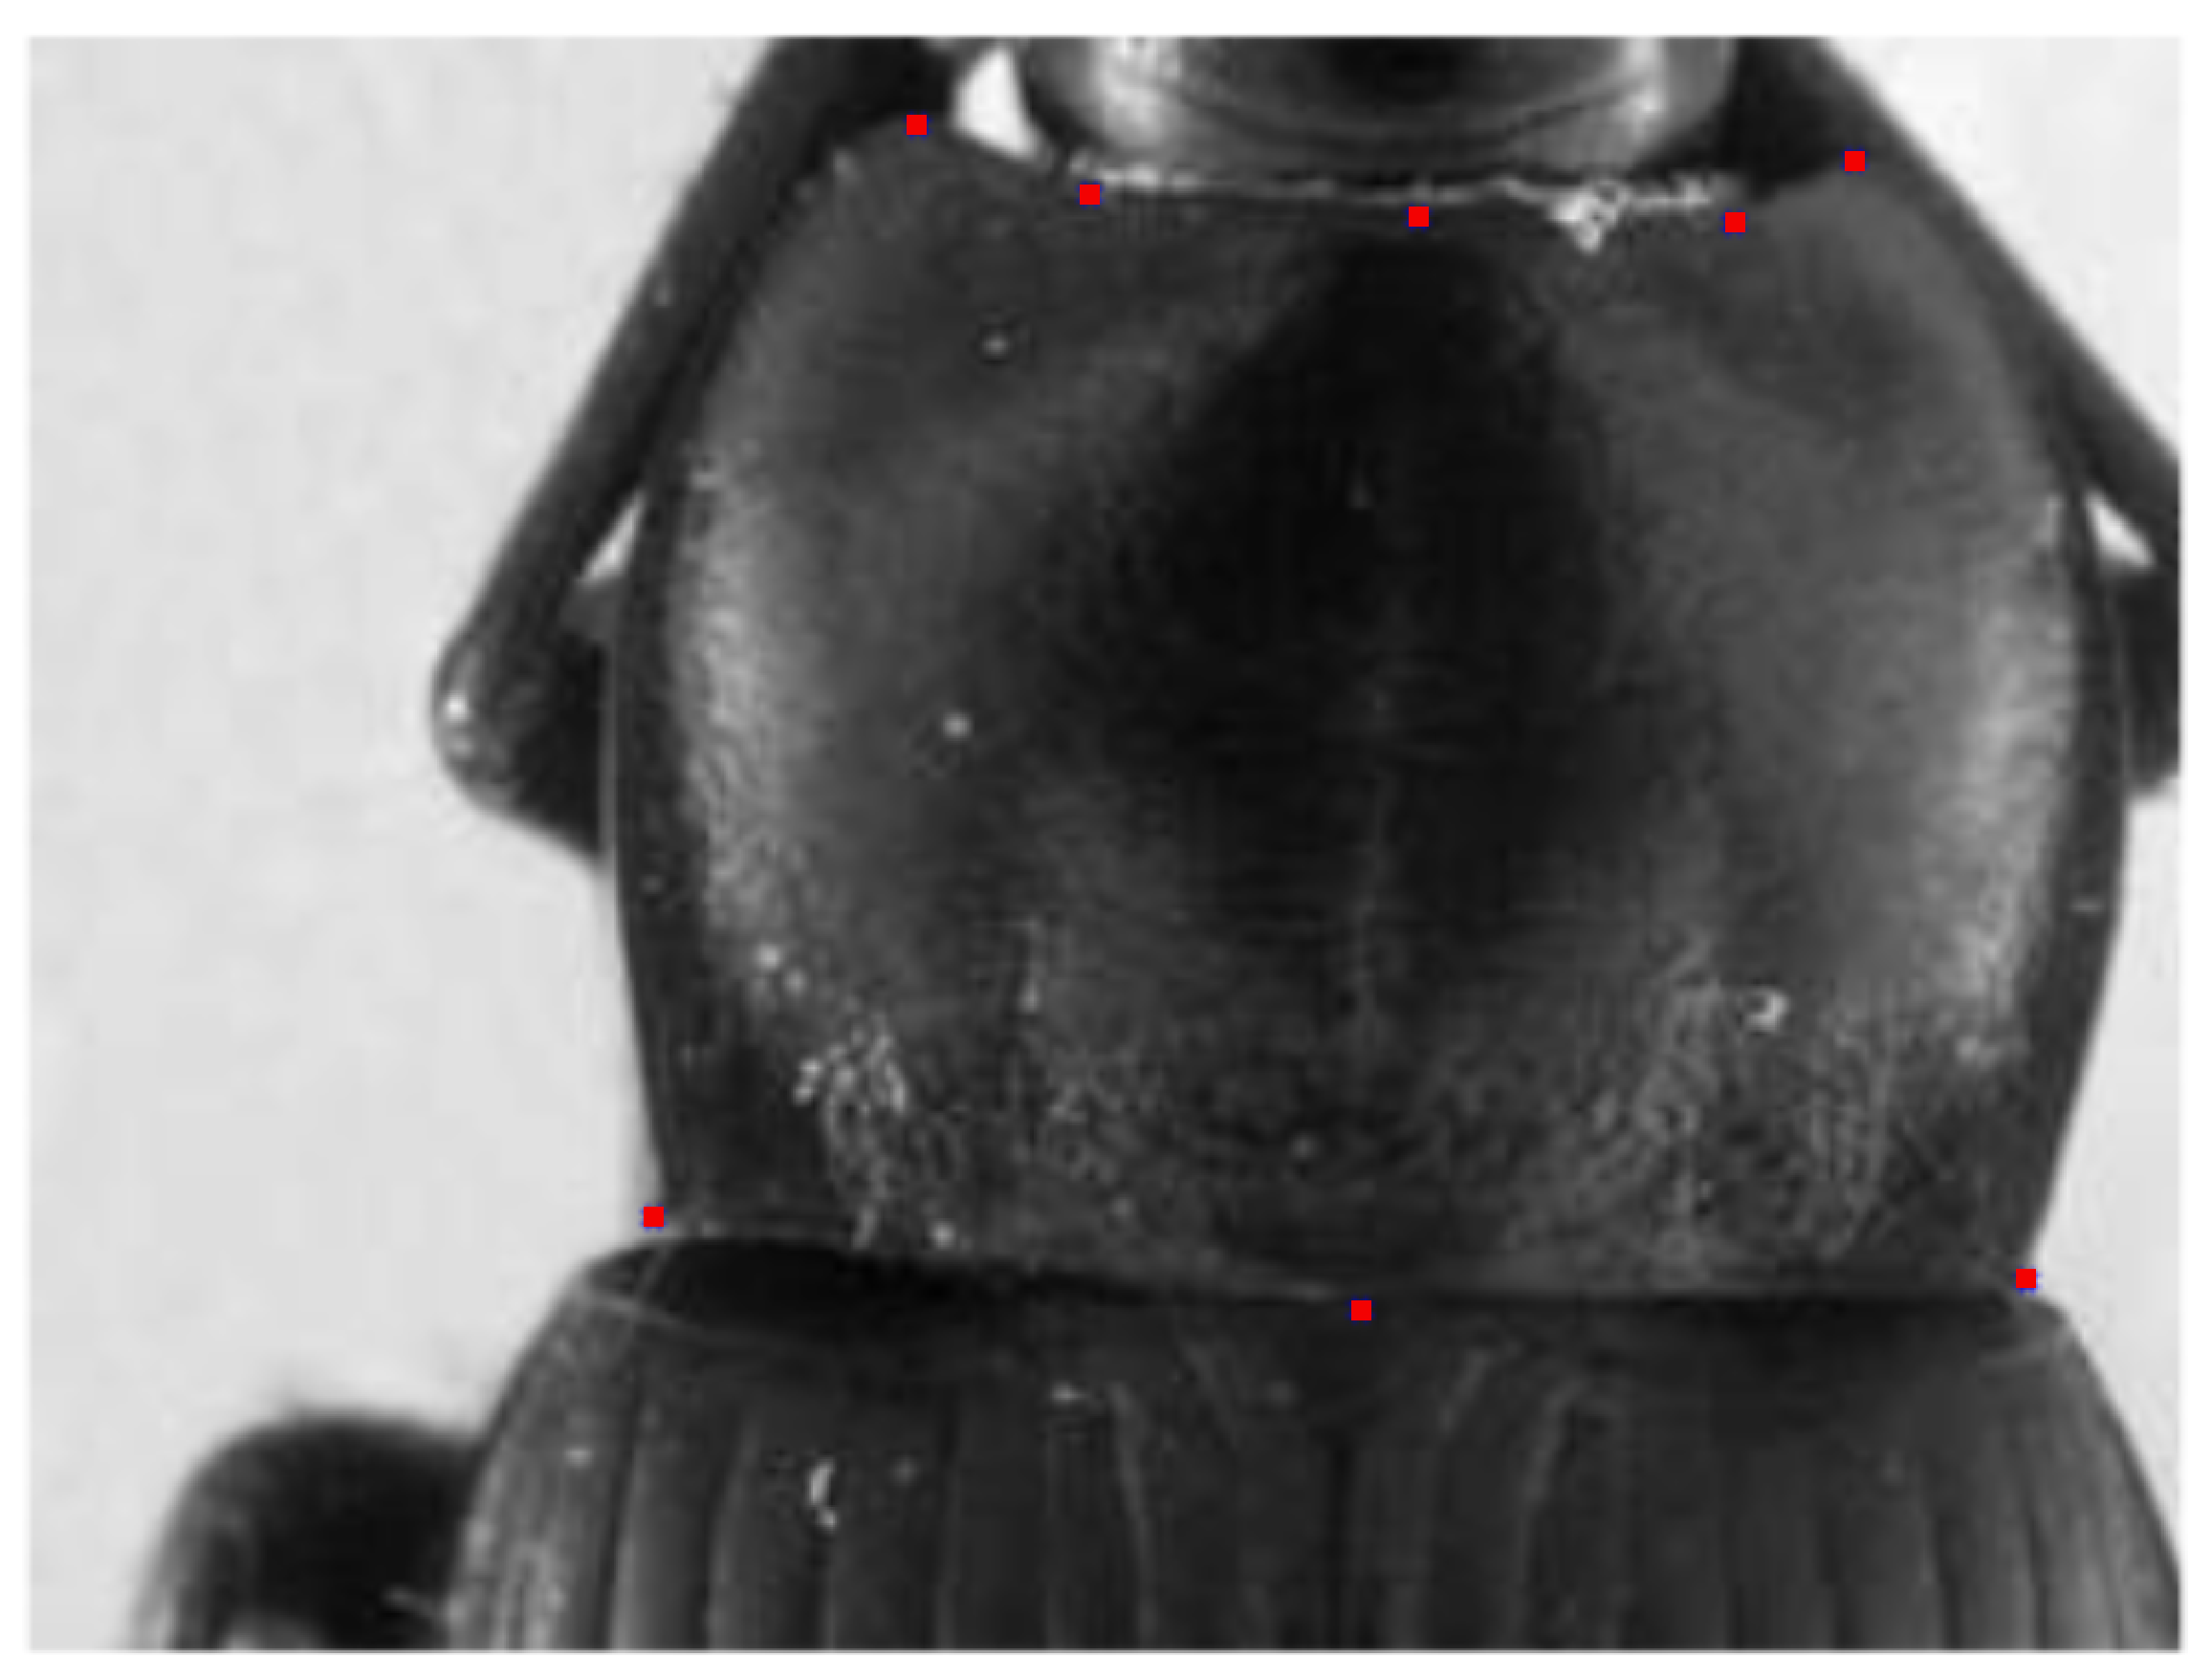
\includegraphics[scale=0.18]{images/plandmark}}
	\caption{The predicted landmarks on an image in test set (red points)}
	\label{figrsexample}
\end{figure}
For a comprehensive evaluation of the efficacy of the network. The correlation coefficient on the coordinates of predicted landmarks is calculated by using three methods: Pearson\cite{pallant2013spss}, Spearman\cite{myers2010research}, and Kendall\cite{kendall1938new}. These results are shown in Table.\ref{tab1}.
\begin{table}[htbp]
\caption{The correlation coefficient of predicted landmarks on several correlation methods}
\begin{center}
\begin{tabular}{|c|c|c|}
\hline
\textbf{Method} & \textbf{x-correlation} & \textbf{y-correlation} \\ \hline
Pearson & 0.9970585 & 0.9978605 \\ \hline
Spearman & 0.9942475 & 0.9859642 \\ \hline
Kendall & 0.9430501 & 0.9067739 \\ \hline
\end{tabular}
\label{tab1}
\end{center}
\end{table}

Besides the coefficient, the distance from predicted landmarks to manual landmarks deserves attention also. Firstly, the distance between them is calculated. Then, the standard deviation\cite{bland1996statistics} is used to quantify the dispersion of a set of distance. Table.\ref{tab2} shows the average error distance given on each landmark. Fig.\ref{figchart} shows the proportion of acceptable landmarks. In our case, a predicted landmark is acceptable if the distance between it and corresponding manual landmarks is less than the average distance plus a value of standard deviation. Most of the landmarks have been detected with the accuracy greater than $70\%$. However, we can see a vast difference between the correlation coefficient results and the proportions on each landmark.

\begin{table}[htbp]
\caption{The average distance on each landmark}
\begin{center}
\begin{tabular}{|c|p{1.5cm}|}
\hline
\textbf{$\#$Landmark} & \textbf{Distance} \\ \hline
1 & 4.002  \\ \hline
2 & 4.4831 \\ \hline
3 & 4.2959 \\ \hline
4 & 4.3865 \\ \hline
5 & 4.2925 \\ \hline
6 & 5.3631 \\ \hline
7 & 4.636 \\ \hline
8 & 4.9363 \\ \hline
\end{tabular}
\label{tab2}
\end{center}
\end{table}

\begin{figure}[htbp]
	\centerline{\includegraphics[scale=0.2]{images/chart}}
	\caption{The proportion of acceptable predicted landmarks}
	\label{figchart}
\end{figure}

At the test phase, the trained network is used to predict the landmarks on a set of unseen images (test set). With a bit of Python code, the program outputs the predicted-landmarks of the images as TPS files; in additional, it also fills and displays the predicted-landmarks on sixteenth firstly images of test data. With the outputs are TPS files, the user can use MAELab\cite{le2017maelab} framework\footnote{MAELab is a free software written in C++. It can be directly
and freely obtained by request at the authors.} to display the landmarks on the images.
\section{Conclusion and future works}
We present a method for landmarks prediction on beetle images, specifically, pronotum images. The method used the convolutional neural network for automatic detection landmarks. It includes three times repeated of a structure consists of a convolutional layer, a max pooling layer, and a dropout layer, followed by the connected layers. During the training phase, the techniques are used to prevent overfitting, a common issue of the neural network. The network was trained in several times in different selection of training data. After training with the manual landmarks which given by the biologist, the network is possible to predict the landmarks on the set of unseen images. The model is implemented using open source tools and available on GitHub.

The results from the testing period are evaluated by several different methods: The correlations have been used to calculate the coefficients on coordinates of predicted landmarks. Besides, the distance between manual landmark and corresponding predicted-landmark were also computed. Then, the standard deviation based on the distance is used to correct the acceptable landmarks. The average of distance errors on each landmark was also considered. Some of the methods have been given the good coefficient. The quality of prediction can be used to replace for manual landmarks in some aspect.

Finally, using the convolutional network to predict the landmarks on biological images promising the good results. However, when we expect more about the accuracy of predicted landmarks, the result of this work is not enough. Therefore, future research in landmarking identification appears as a improve the worth exploring.

%\begin{thebibliography}{00}
%\bibitem{b1} G. Eason, B. Noble, and I. N. Sneddon, ``On certain integrals of Lipschitz-Hankel type involving products of Bessel functions,'' Phil. Trans. Roy. Soc. London, vol. A247, pp. 529--551, April 1955.
%\bibitem{b2} J. Clerk Maxwell, A Treatise on Electricity and Magnetism, 3rd ed., vol. 2. Oxford: Clarendon, 1892, pp.68--73.
%\bibitem{b3} I. S. Jacobs and C. P. Bean, ``Fine particles, thin films and exchange anisotropy,'' in Magnetism, vol. III, G. T. Rado and H. Suhl, Eds. New York: Academic, 1963, pp. 271--350.
%\bibitem{b4} K. Elissa, ``Title of paper if known,'' unpublished.
%\bibitem{b5} R. Nicole, ``Title of paper with only first word capitalized,'' J. Name Stand. Abbrev., in press.
%\bibitem{b6} Y. Yorozu, M. Hirano, K. Oka, and Y. Tagawa, ``Electron spectroscopy studies on magneto-optical media and plastic substrate interface,'' IEEE Transl. J. Magn. Japan, vol. 2, pp. 740--741, August 1987 [Digests 9th Annual Conf. Magnetics Japan, p. 301, 1982].
%\bibitem{b7} M. Young, The Technical Writer's Handbook. Mill Valley, CA: University Science, 1989.

%\end{thebibliography}
\bibliographystyle{IEEEtran}
\bibliography{includes/references}
\section*{Appendix}
The proposed network consists 13 layers of convolutional, max-pooling, dropout and full-connected layers. The layers are interleaved arrangement as discussed in section \ref{sec3}. In which:
\begin{itemize}
	\item Input size: $1 \times 256 \times 192$
	\item Convolutional layers: 3 layers
	\item Max pooling layers: 3 layers
	\item Dropout layers: 4 layers
	\item Full-connected layers: 3 layers
\end{itemize}


The detail parameters in each layer are shown in Table \ref{modelparameters}.
\begin{table}[htbp]
	\caption{The parameters at each layer of the proposed network}
	\centering
	\begin{tabular}{| l |  p{4cm} | }
	\hline
		Layers &  Type of layer and parameters  \\ \hline
		input & $1 \times 256 \times 192$ \\ \hline
 		layer 1 & CONV(32,3,1,0) \\ \hline
		layer 2 & POOL(2,2,0) \\ \hline
		layer 3 & \textbf{DROP(0.1)} \\ \hline
		layer 4 & CONV(64,2,1,0) \\ \hline
		layer 5 & POOL(2,2,0) \\ \hline
		layer 6 & \textbf{DROP(0.2)} \\ \hline
		layer 7 & CONV(128,2,1,0) \\ \hline
		layer 8 & POOL(2,2,0) \\ \hline
		layer 9 & \textbf{DROP(0.3)} \\ \hline
		layer 10 & FC(1000) \\ \hline
		layer 11 & \textbf{DROP(0.5)} \\ \hline
		layer 12& FC(1000) \\ \hline
		layer 13 & FC(16) \\ \hline
	\end{tabular}
	\label{modelparameters}
\end{table}~\\[1cm]
Which:
\begin{itemize}
	\item CONV(x,y,z,t): convolutional layer with the parameters: \textit{x = number of filters, y = size of filter matrix, z = stride value, t = padding value}
	\item POOL(y,z,t): maximum pooling layer with: \textit{y = size of filter, z = stride value, t = padding value}
	\item DROP(p): dropout layer with \textit{p is the dropout ratio}
	\item FC(x): full-connected layer with \textit{x is the number of output}
\end{itemize}
\end{document}
